\problemname{Insertion Order}

A friend of yours is currently taking a class on algorithms and data
structures. Just last week he learned about binary search trees and
the importance of using self-balancing trees in order to keep the tree
height low and guarantee fast access to every node.

Recall that a binary search tree is a binary tree with each node
storing a key, and the property that the key of each node is greater
than all keys in the left subtree of that node and less than all keys
in the right subtree. A new key is inserted into the tree by adding a
new leaf node with that key in the only position such that the
property is maintained, as seen in the figure below.

\begin{figure}[!h]
  \centering
  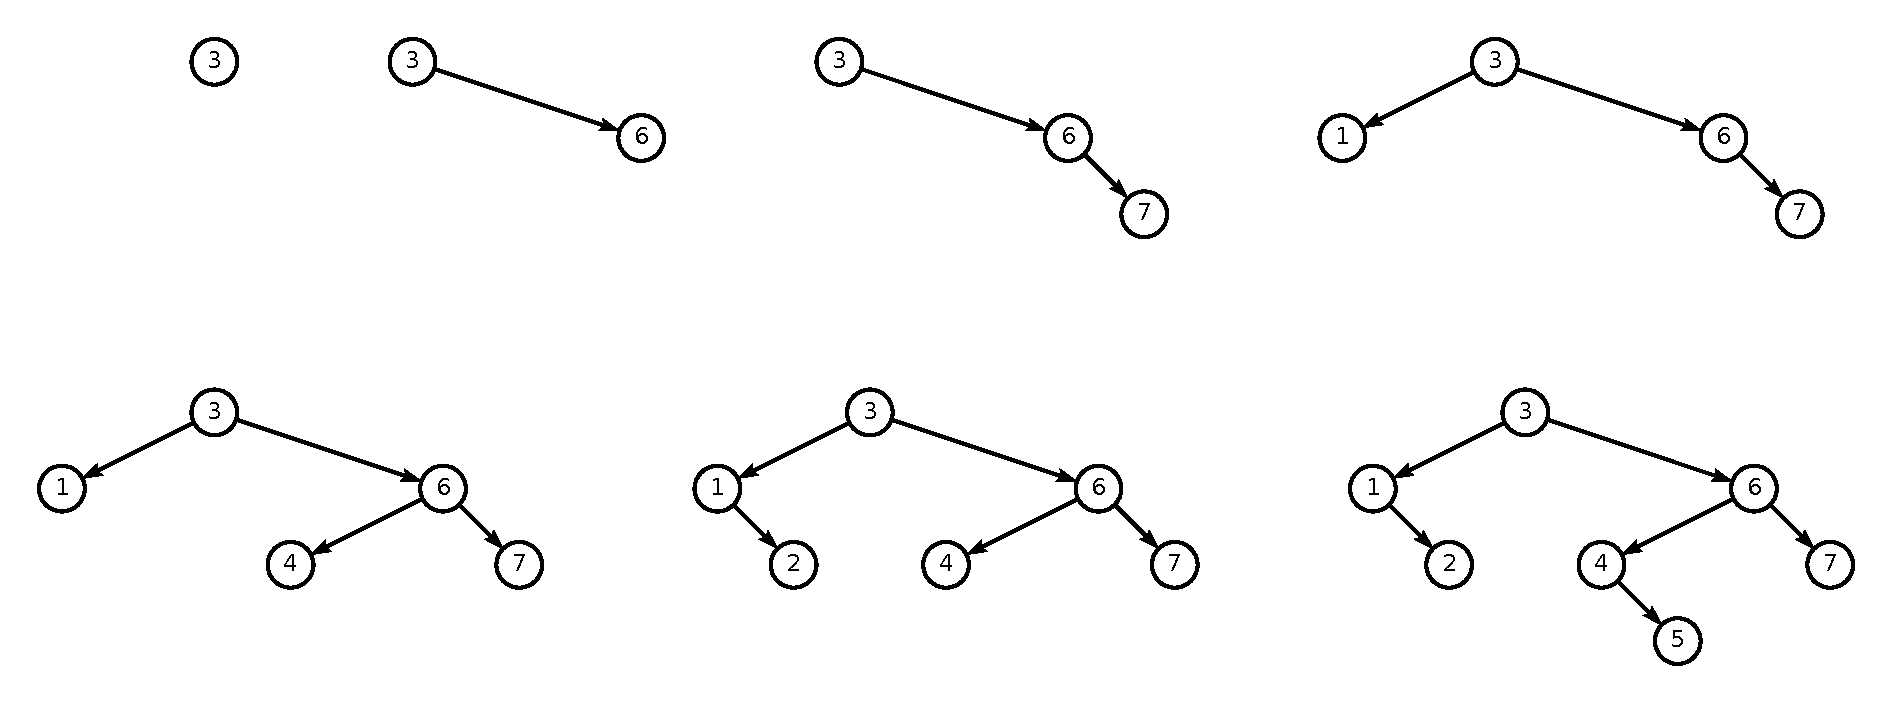
\includegraphics[width=0.99\textwidth]{illustration}
  \caption{Illustration of the first sample case.}
\end{figure}

To illustrate to him just how bad things can get without
self-balancing, you want to show him that it is possible to build
trees of nearly any height by carefully choosing an insertion order.

You are given two integers $n$ and $k$ and want to construct a binary
search tree with $n$ nodes of height $k$ (the height of a tree is the
maximal number of nodes on a path from the root to a leaf).
To do so, you need to find a permutation of the integers from $1$ to
$n$ such that, when they are inserted into an empty binary search tree
in that order (without self-balancing), the resulting tree has height
$k$.

\section*{Input} 

The input consists of two integers $n$ and $k$
($1 \le k \le n \le 2\cdot10^5$), where $n$ is the number of nodes in
the tree and $k$ is the exact height the tree should have.

\section*{Output} 

If there is no solution, output \texttt{impossible}. Otherwise, output
one line with $n$ integers, the requested permutation. If there is
more than one solution, any one of them will be accepted.
